\documentclass[documentation.tex]{subfiles}
\begin{document}

\subsection{Общ поглед върху интерфейса} \label{interface}
    \begin{text}\par
    По-долу е паказан фрагмент от код, показващ начина на употреба на WebFrame++\cite{webframe}.
    \end{text}\\
    {\centering
    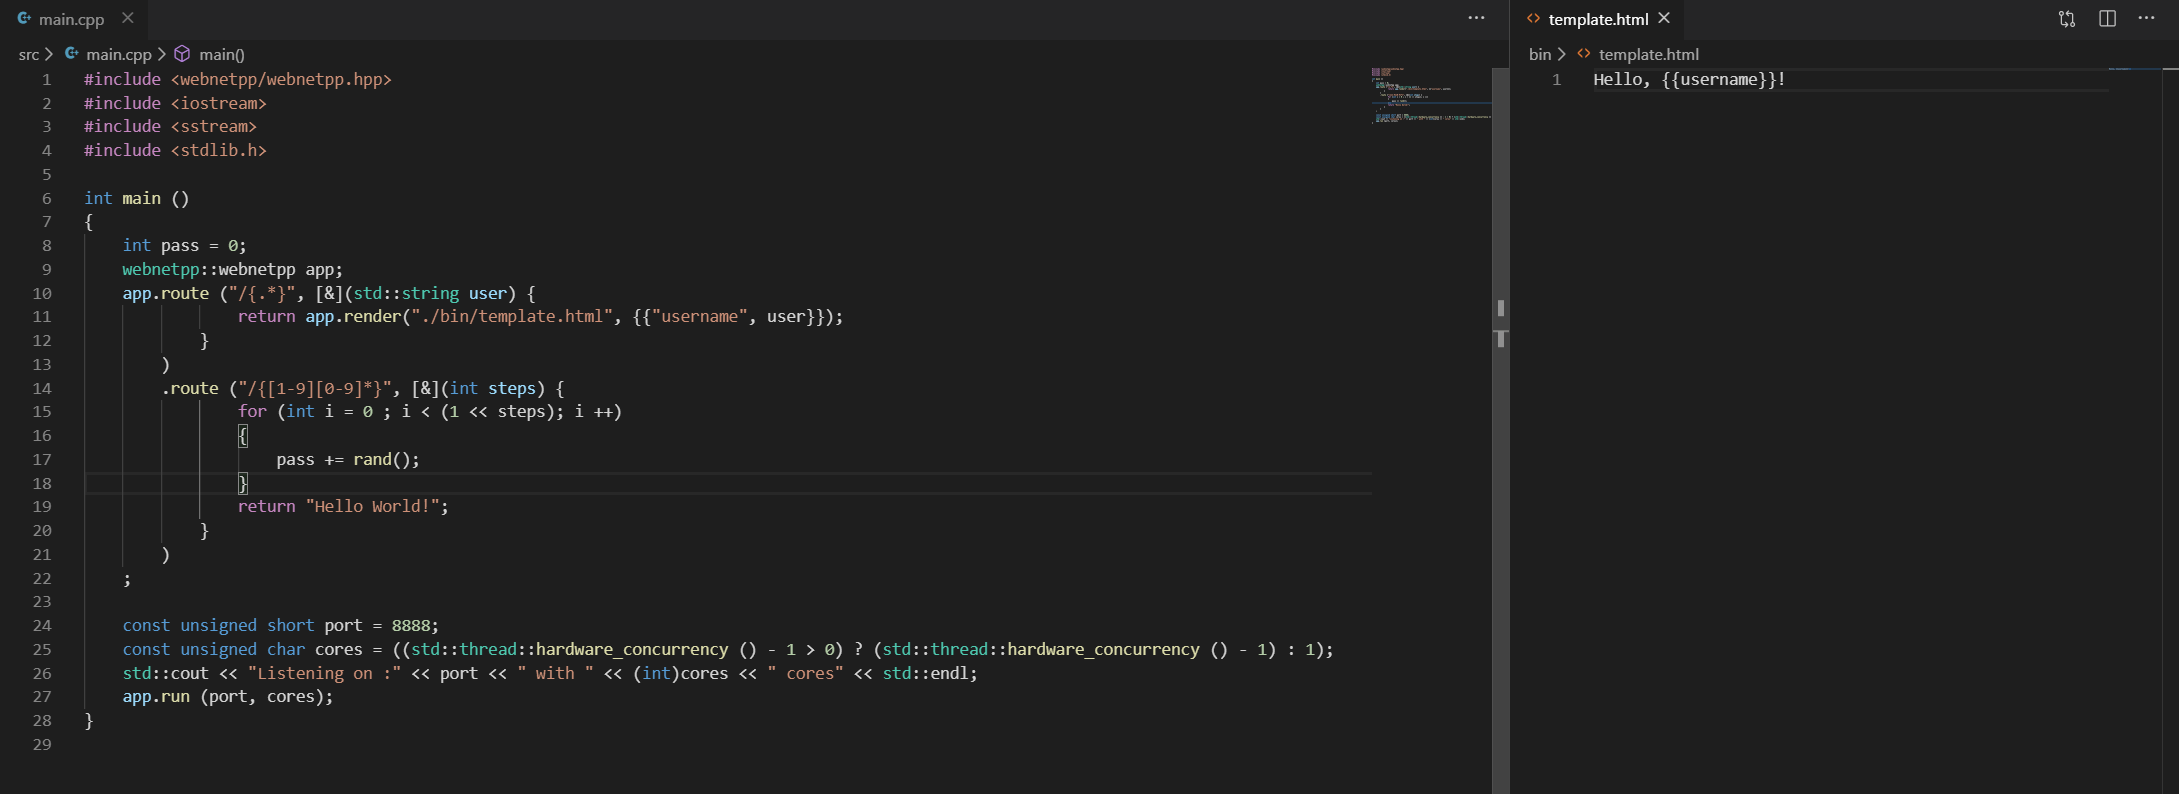
\includegraphics[width=1\textwidth]{images/new_version.png}
    }
\subsection{Flask - Python}
    \begin{text}\par
    По-долу е паказан фрагмент от код, показващ начина на употреба на конкурента Flask Framework за Python.
    \end{text}\\
    {\centering
    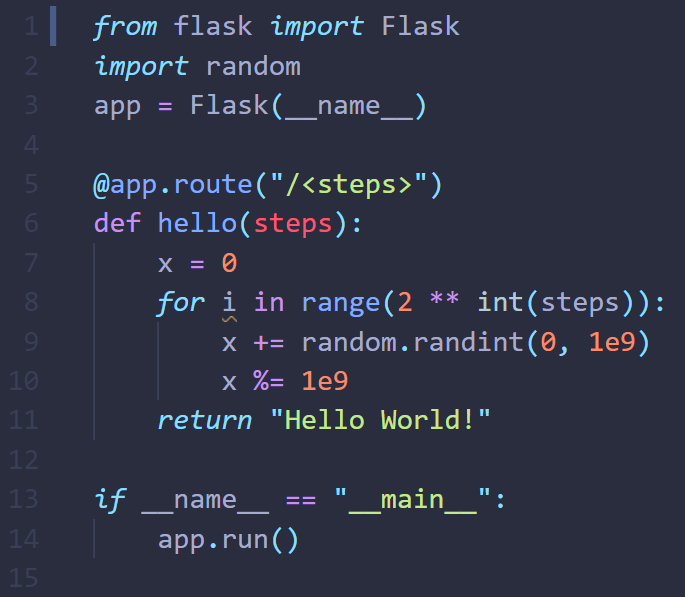
\includegraphics[width=0.75\textwidth]{images/flask.png}
    }
\subsection{Express - Node.JS}
    \begin{text}\par
    По-долу е паказан фрагмент от код, показващ начина на употреба на конкурента Express за Node.JS.
    \end{text}\\
    {\centering
    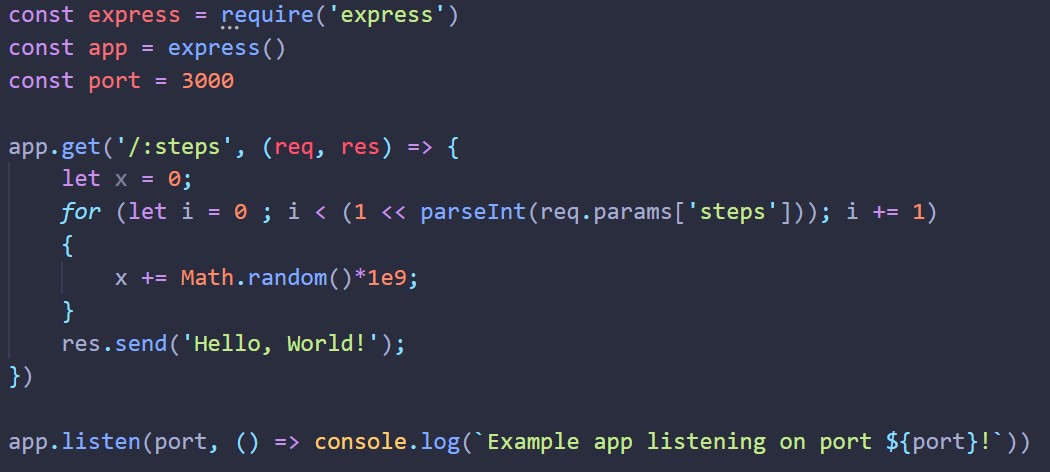
\includegraphics[width=1\textwidth]{images/nodejs.png}
    }
\subsection{Извод}
    \begin{text}\par
        Библиотеката наподобява най-разпространените в световен мащаб библиотеки за разработка на уеб приложения.
    \end{text}
    
    {\centering
    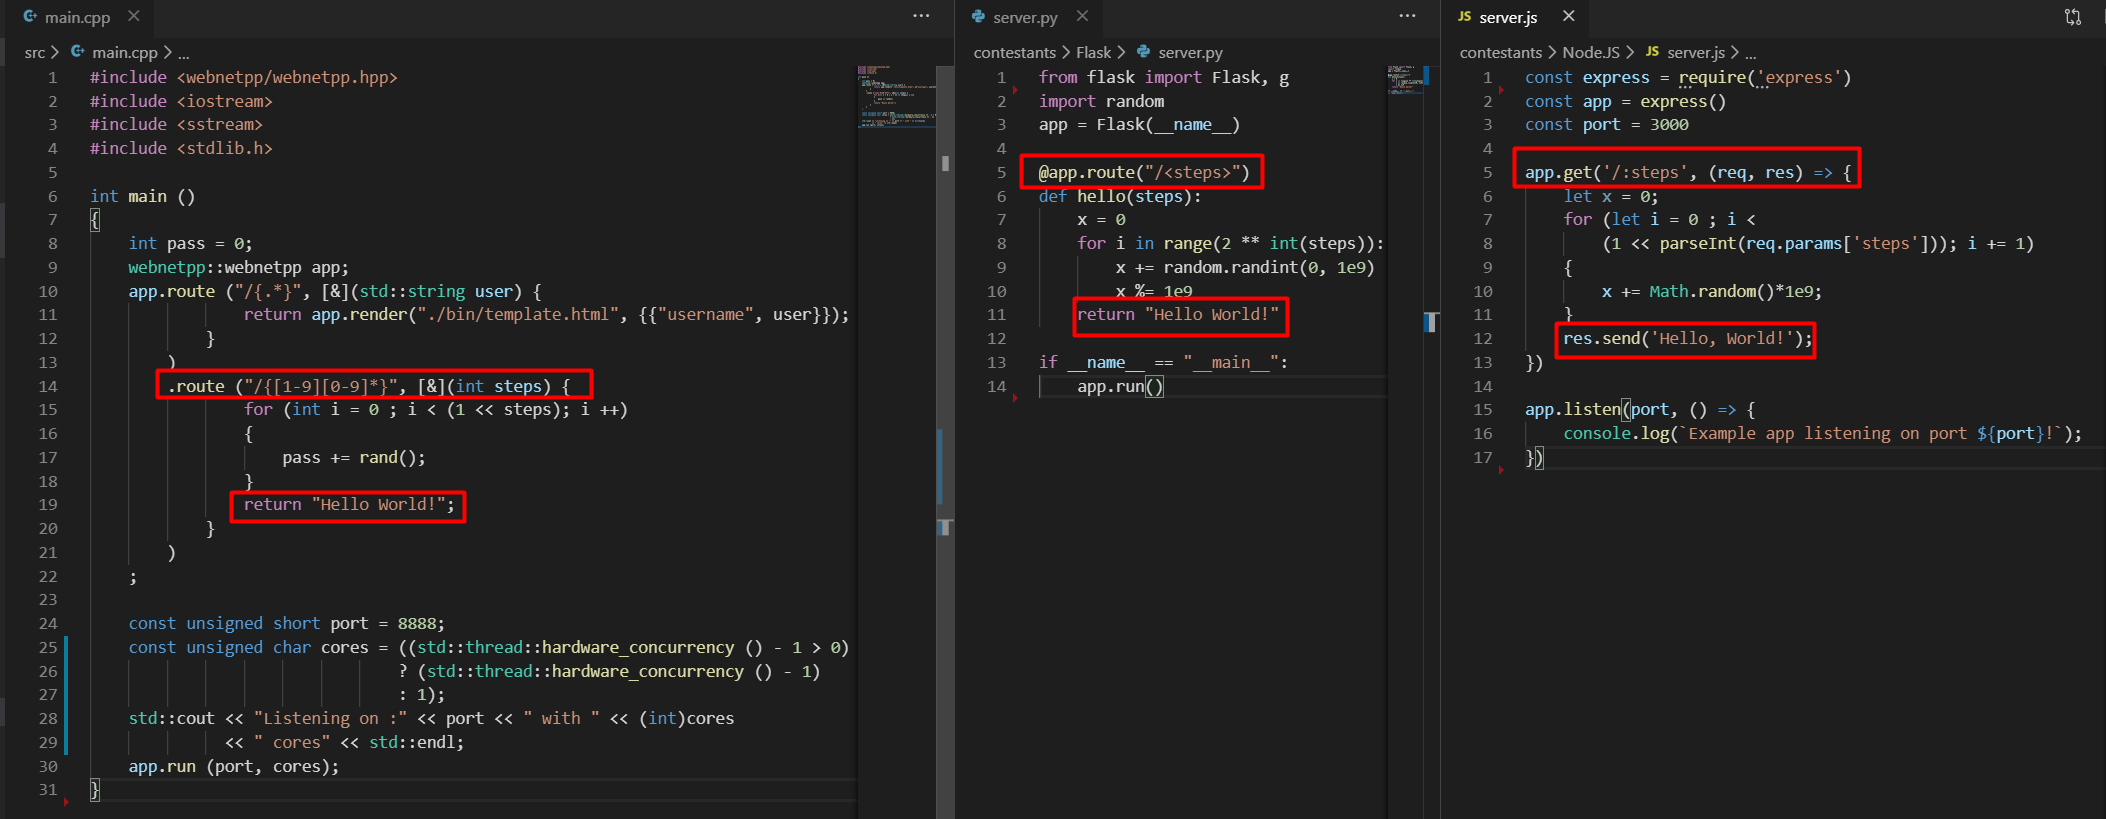
\includegraphics[width=1.2\textwidth]{images/all_new.png}
    }
    
    \begin{text}\par
        Библиотеката те първа ще се опрастява още и още. Към момента има повечето от възможностите на лидерите в областта и има допълнителни опции, които услесняват програмиста и му спестяват доста проверки за валидност на данните.
    \end{text}
\end{document}